%%%%%%%%%%%%%%%%%%%%%%%%%%%%%%%%%%%%%%%%%%  不使用 authblk 包制作标题  %%%%%%%%%%%%%%%%%%%%%%%%%%%%%%%%%%%%%%%%%%%%%%
%-------------------------------PPT Title-------------------------------------
\title{{\rm WIEN2k}算例举要}
%-----------------------------------------------------------------------------
%----------------------------Author & Date------------------------------------

%\author[\textrm{Jun\_Jiang}]{姜\;\;骏\inst{}} %[]{} (optional, use only with lots of authors)
%% - Give the names in the same order as the appear in the paper.
%% - Use the \inst{?} command only if the authors have different
%%   affiliation.
%\institute[BCC]{\inst{}%
\institute[Gain~Strong]{\inst{}%
%\vskip -20pt 北京市计算中心~云平台事业部~~姜骏}
\vskip -20pt {\large 格致斯创~科技}}
\date[\today] % (optional, should be abbreviation of conference name)
{%	{\fontsize{6.2pt}{4.2pt}\selectfont{\textcolor{blue}{E-mail:~}\url{jiangjun@bcc.ac.cn}}}
\vskip 45 pt {\fontsize{8.2pt}{6.2pt}\selectfont{%清华大学\;\;物理系% 报告地点
%	\vskip 5 pt \textrm{2016.07.29-31}
}}
}

%% - Either use conference name or its abbreviation
%% - Not really information to the audience, more for people (including
%%   yourself) who are reading the slides onlin%%   yourself) who are reading the slides onlin%%   yourself) who are reading the slides onlineee
%%%%%%%%%%%%%%%%%%%%%%%%%%%%%%%%%%%%%%%%%%%%%%%%%%%%%%%%%%%%%%%%%%%%%%%%%%%%%%%%%%%%%%%%%%%%%%%%%%%%%%%%%%%%%%%%%%%%%

\subject{}
% This is only inserted into the PDF information catalog. Can be left
% out.
%\maketitle
\frame
{
%	\frametitle{\fontsize{9.5pt}{5.2pt}\selectfont{\textcolor{orange}{“高通量并发式材料计算算法与软件”年度检查}}}
\titlepage
}
%-----------------------------------------------------------------------------

%------------------------------------------------------------------------------列出全文 outline ---------------------------------------------------------------------------------
\section{\rm{WIEN2k}计算举例}
\frame
{
	\frametitle{\textrm{WIEN2k}算例:~\textrm{case.structure}}
\vspace*{-18pt}
\begin{minipage}[t]{0.39\textwidth}
\begin{figure}[h!]
\centering
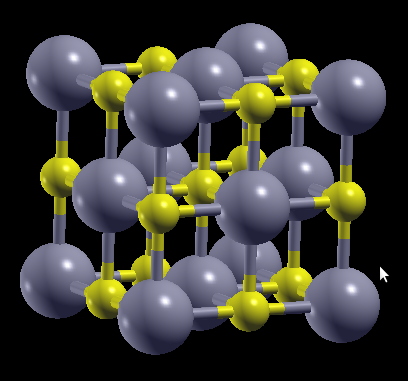
\includegraphics[width=1.5in]{Figures/WIEN2k_TiC.png}
\caption{\tiny \textrm{The structure of TiC.}}%(与文献\cite{EPJB33-47_2003}图1对比)
\label{Fig:WIEN2k_TiC}
\end{figure}
\end{minipage}
\hfill
\begin{minipage}[t]{0.59\textwidth}
\begin{figure}[h!]
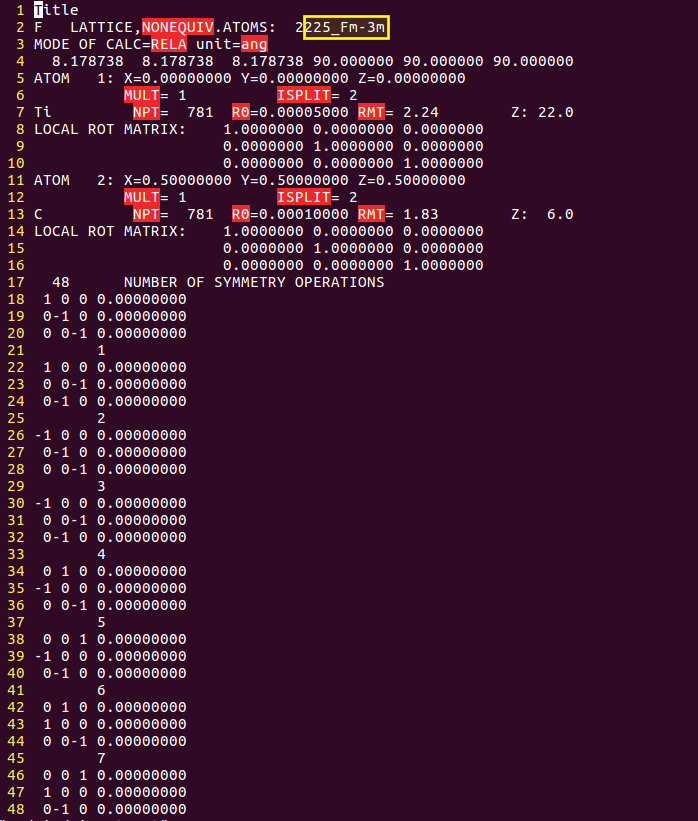
\includegraphics[height=2.95in]{Figures/WIEN2k_TiC-structure.png}
%\caption{\tiny Breakup of a submesh cell into six tetrahedra.}%(与文献\cite{EPJB33-47_2003}图1对比)
\label{Fig:WIEN2k_TiC-structure}
\end{figure}
\end{minipage}
}

\frame
{
	\frametitle{\textrm{WIEN2k}算例:~\textrm{case.structure}}
\vspace*{-17pt}
\begin{minipage}[t]{0.39\textwidth}
\begin{figure}[h!]
\centering
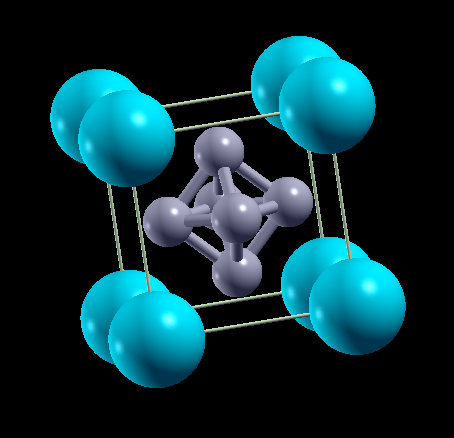
\includegraphics[width=1.5in]{Figures/WIEN2k_CaB6.png}
\caption{\tiny \textrm{The structure of \ch{CaB6}.}}%(与文献\cite{EPJB33-47_2003}图1对比)
\label{Fig:WIEN2k_CaB6}
\end{figure}
\end{minipage}
\hfill
\begin{minipage}[t]{0.59\textwidth}
\begin{figure}[h!]
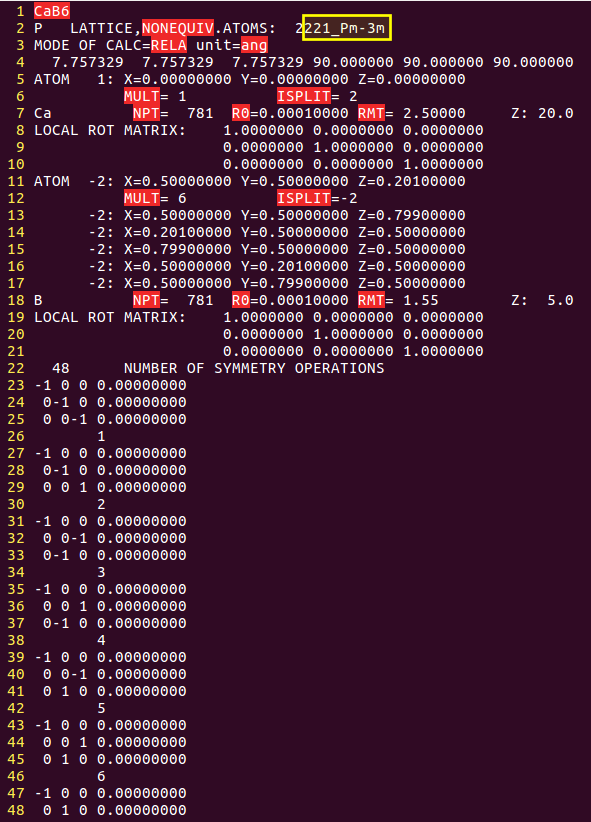
\includegraphics[height=2.95in]{Figures/WIEN2k_CaB6-structure.png}
%\caption{\tiny Breakup of a submesh cell into six tetrahedra.}%(与文献\cite{EPJB33-47_2003}图1对比)
\label{Fig:WIEN2k_CaB6-structure}
\end{figure}
\end{minipage}
}

\frame
{
\frametitle{\textrm{WIEN2k}中自洽迭代的流程组织}
\begin{figure}[h!]
\centering
\hspace*{-10pt}
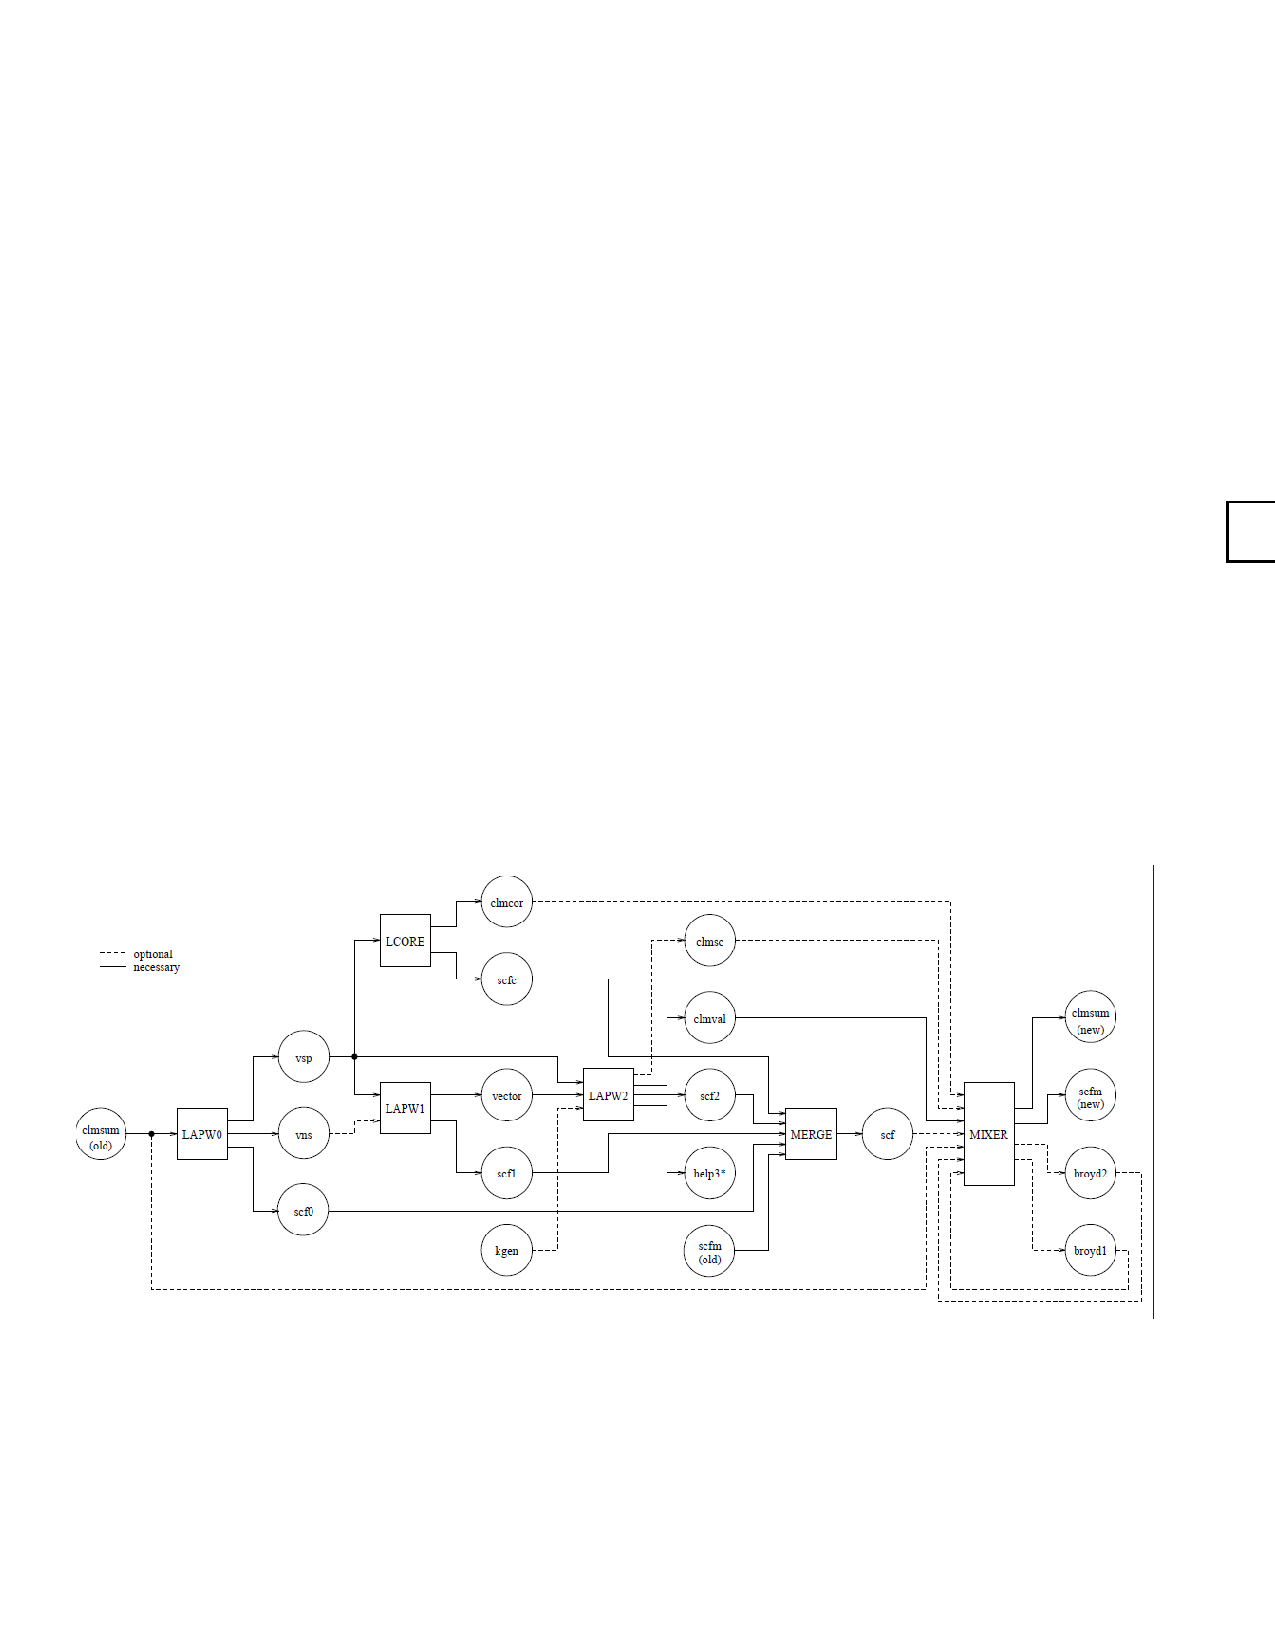
\includegraphics[height=1.72in,width=4.2in,viewport=30 165 550 375,clip]{Figures/WIEN2k_Data_flow.pdf}
\caption{\tiny \textrm{Data flow during a SCF cycle (programX.def, case.struct, case.inX, case.outputX and optional files are omitted).}}%(与文献\cite{EPJB33-47_2003}图1对比)
\label{WIEN2k_Data_flow}
\end{figure}
}

\frame
{
	\frametitle{\textrm{WIEN2k}计算示范:~\textrm{SCF}}
\vspace*{-13pt}
\begin{figure}[h!]
\centering
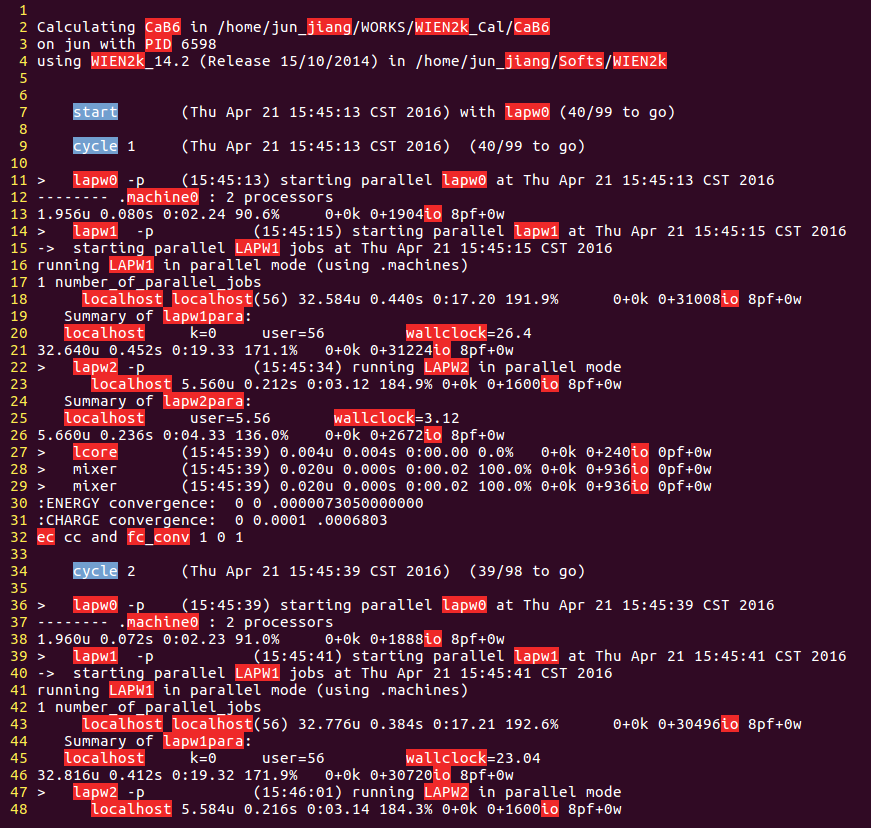
\includegraphics[height=2.98in]{Figures/WIEN2k_CaB6-SCF.png}
%\caption{\tiny \textrm{The structure of TiC.}}%(与文献\cite{EPJB33-47_2003}图1对比)
\label{Fig:WIEN2k_SCF}
\end{figure}
}

\frame
{
	\frametitle{\textrm{WIEN2k}计算示范:~\ch{\textrm{CaB6}}的总能量}
\vspace*{-25pt}
\begin{figure}[h!]
\centering
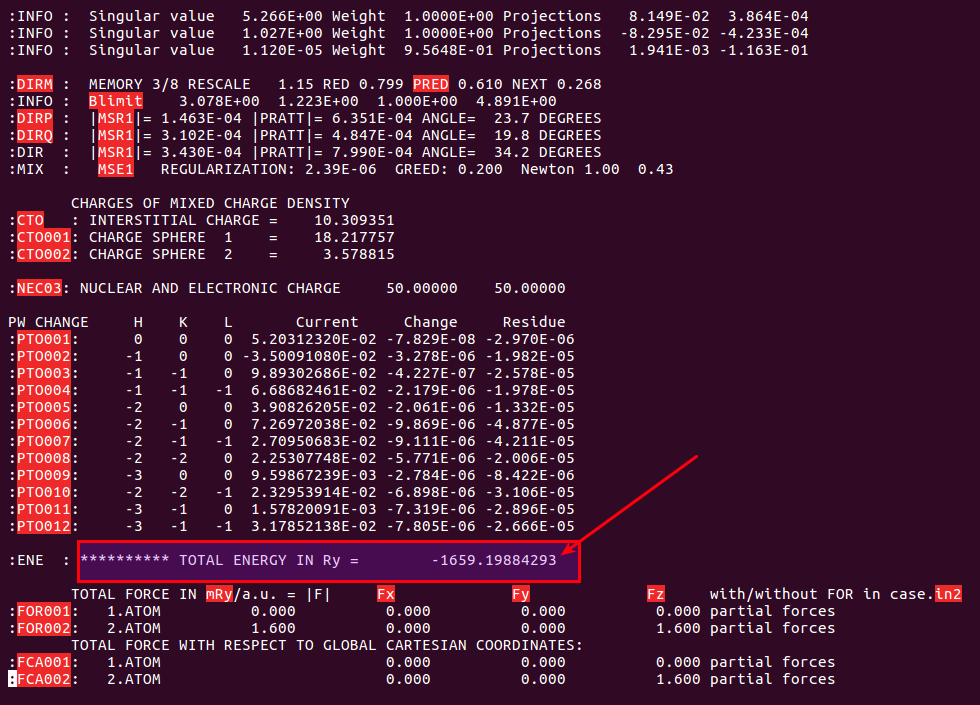
\includegraphics[height=2.98in]{Figures/WIEN2k_CaB6-TotEne.png}
%\caption{\tiny \textrm{The structure of TiC.}}%(与文献\cite{EPJB33-47_2003}图1对比)
\label{Fig:WIEN2k_TotEne}
\end{figure}
}

\frame
{
	\frametitle{\textrm{WIEN2k}计算示范:~\ch{\textrm{CaB6}}的能量本征值}
\vspace*{-14pt}
\begin{figure}[h!]
\centering
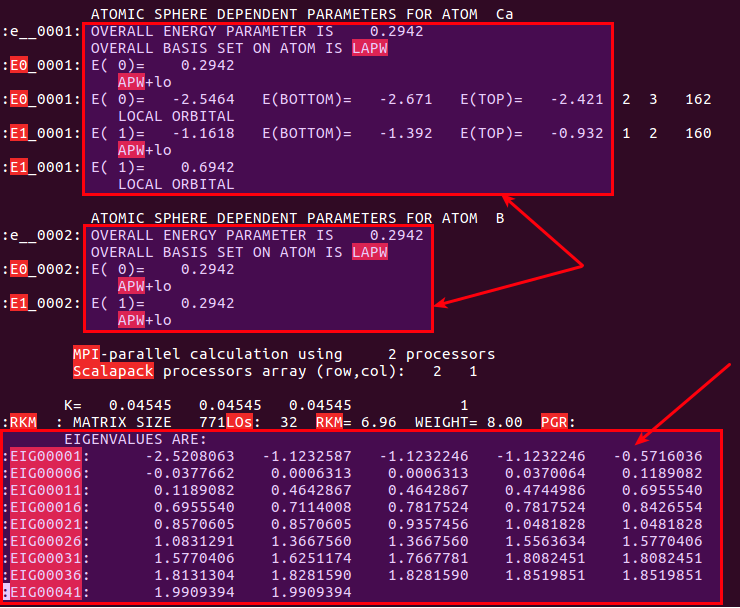
\includegraphics[height=2.98in]{Figures/WIEN2k_CaB6-EigVal.png}
%\caption{\tiny \textrm{The structure of TiC.}}%(与文献\cite{EPJB33-47_2003}图1对比)
\label{Fig:WIEN2k_EigVal}
\end{figure}
}

\frame
{
	\frametitle{\textrm{WIEN2k}算例:~基函数的选择}
\begin{figure}[h!]
	\vspace{-15pt}
\centering
\hspace{15pt}
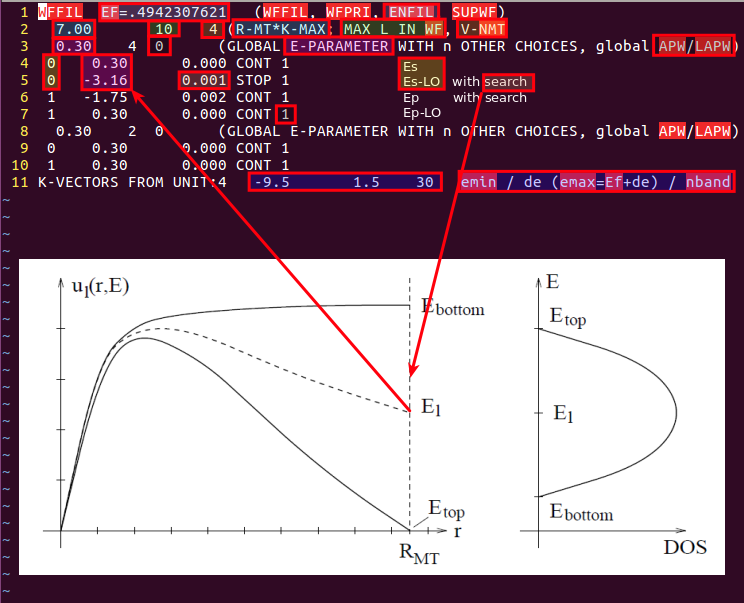
\includegraphics[height=2.55in,width=3.35in,viewport=10 30 750 605,clip]{Figures/WIEN2k-in1.png}
\caption{\tiny \textrm{The parameter $\mathrm{E}_l$ in case.in1 for WIEN2k.}}%(与文献\cite{EPJB33-47_2003}图1对比)
\label{WIEN2k-in1}
\end{figure}
}

\frame
{
	\frametitle{\textrm{WIEN2k}计算示范:~\ch{\textrm{CaB6}}的\textrm{Fermi}能}
\vspace*{-25pt}
\begin{figure}[h!]
\centering
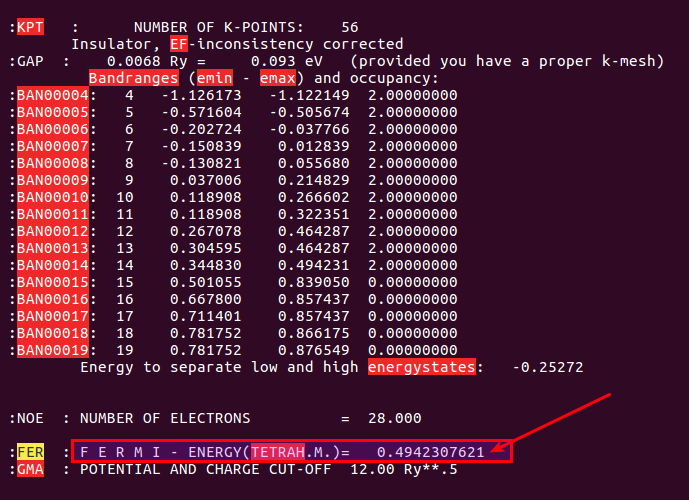
\includegraphics[height=2.98in]{Figures/WIEN2k_CaB6-Fermi.png}
%\caption{\tiny \textrm{The structure of TiC.}}%(与文献\cite{EPJB33-47_2003}图1对比)
\label{Fig:WIEN2k_Fermi}
\end{figure}
}

\frame
{
	\frametitle{\textrm{WIEN2k}计算示范:~\ch{\textrm{CaB6}}的\textrm{DOS}}
\vspace*{-13pt}
\begin{figure}[h!]
\centering
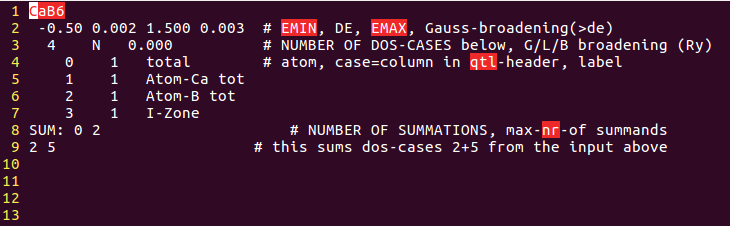
\includegraphics[width=2.8in]{Figures/WIEN2k_CaB6-int.png}
\caption{\tiny \textrm{case.int}}%(与文献\cite{EPJB33-47_2003}图1对比)
\label{Fig:WIEN2k_int}
\end{figure}
\begin{figure}[h!]
\centering
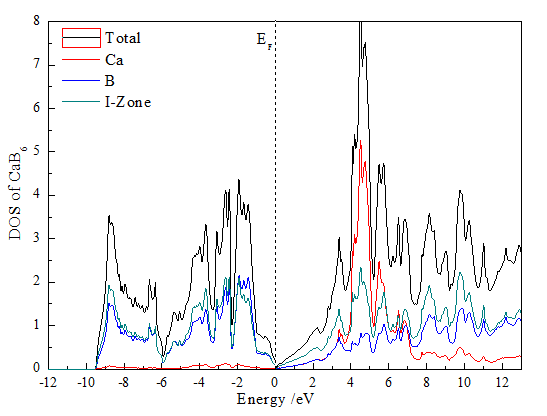
\includegraphics[height=1.60in,width=2.60in]{Figures/WIEN2k_CaB6-DOS.png}
%\caption{\tiny \textrm{The structure of TiC.}}%(与文献\cite{EPJB33-47_2003}图1对比)
\label{Fig:WIEN2k_DOS}
\end{figure}
}

\frame
{
	\frametitle{\textrm{WIEN2k}算例:~能带计算文件}
\vspace*{-5pt}
\begin{minipage}[t]{0.52\textwidth}
\begin{figure}[h!]
\centering
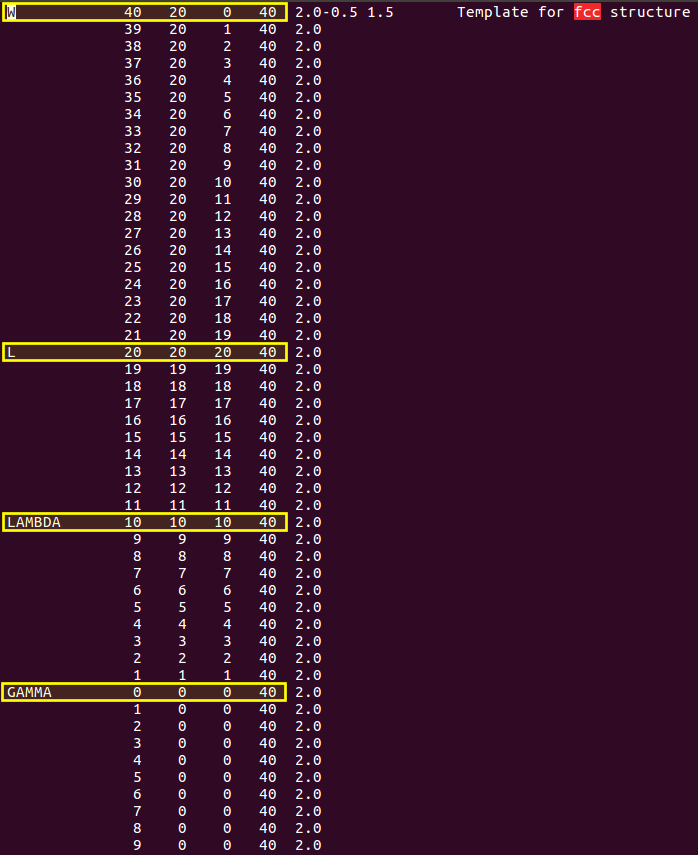
\includegraphics[width=2.0in]{Figures/WIEN2k_CaB6-klist_band.png}
\caption{\tiny \textrm{case.klist\_band}}%(与文献\cite{EPJB33-47_2003}图1对比)
\label{Fig:WIEN2k_CaB6-klist_band}
\end{figure}
\end{minipage}
\hskip 0.2pt
\begin{minipage}[t]{0.46\textwidth}
\begin{figure}[h!]
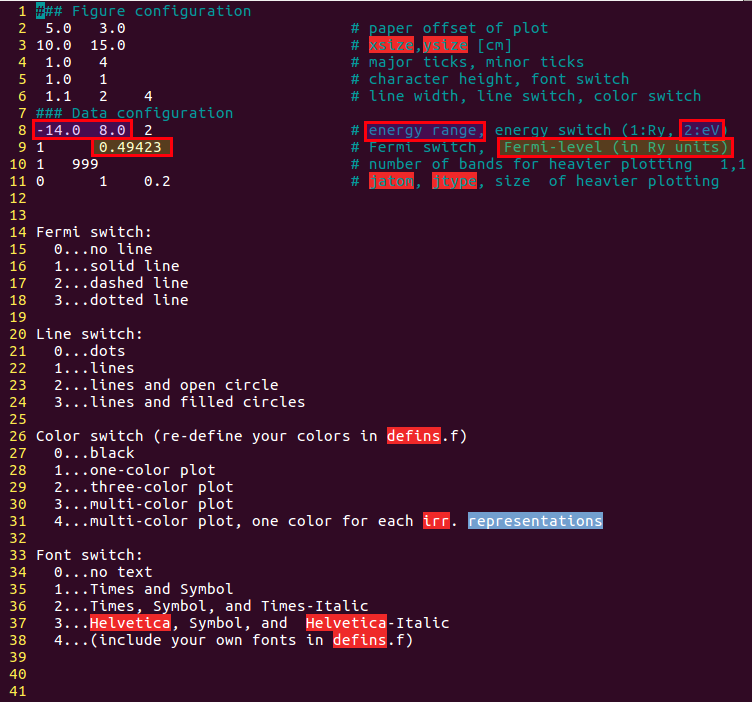
\includegraphics[height=1.9in]{Figures/WIEN2k_CaB6-insp.png}
\caption{\tiny \textrm{case.insp}}%(与文献\cite{EPJB33-47_2003}图1对比)
\label{Fig:WIEN2k_CaB6-insp}
\end{figure}
\end{minipage}
}

\frame
{
	\frametitle{\textrm{WIEN2k}计算示范:~\ch{\textrm{CaB6}}的能带结构}
\vspace*{-13pt}
\begin{figure}[h!]
\centering
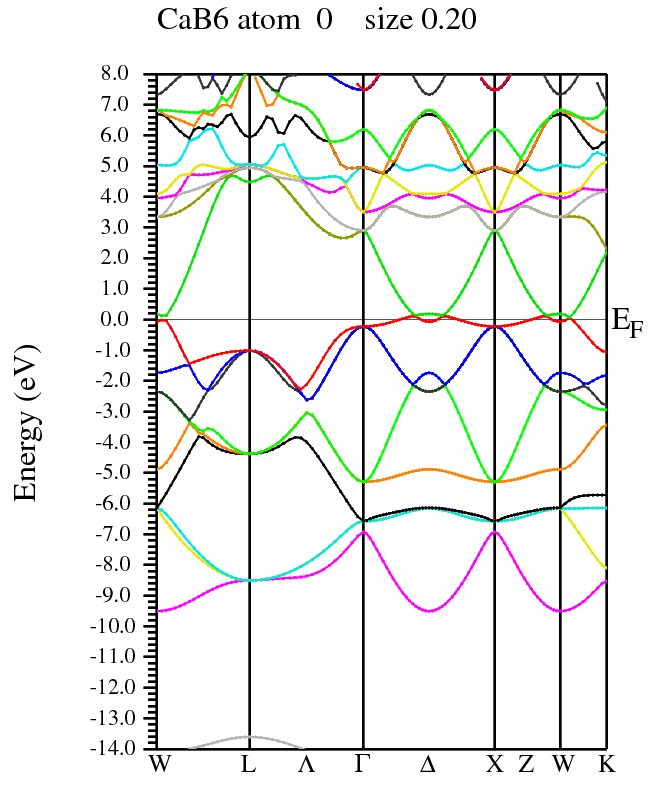
\includegraphics[height=2.98in, viewport=0 10 730 740,clip]{Figures/WIEN2k_CaB6-Band.png}
%\caption{\tiny \textrm{The structure of TiC.}}%(与文献\cite{EPJB33-47_2003}图1对比)
\label{Fig:WIEN2k_Band}
\end{figure}
}

\frame
{
	\frametitle{\textrm{WIEN2k}计算示范:~\ch{\textrm{Cr}}的反铁磁计算}
\vspace*{-18pt}
\begin{figure}[h!]
\centering
\subfigure[\tiny{\textrm{Structure of Cr}}]{
\label{Fig:WIEN2k_BCC-Cr}
	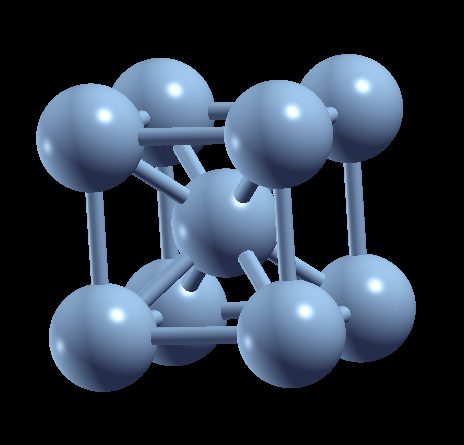
\includegraphics[height=1.20in]{Figures/WIEN2k_BCC_Cr.png}}\\
\subfigure[\tiny{\textrm{Structure of BCC Cr}}]{
\label{Fig:WIEN2k_AFM-Cr-1}
	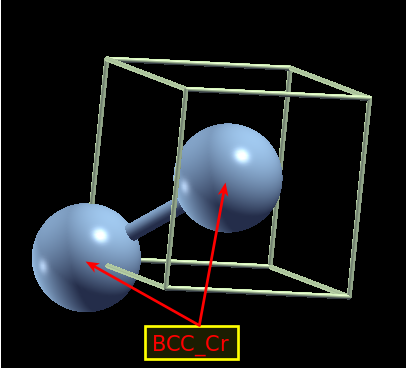
\includegraphics[height=1.20in]{Figures/WIEN2k_BCC_Cr-2.png}}
	\subfigure[\tiny{\textrm{Structure of PCC Cr}}]{
\label{Fig:WIEN2k_AFM-Cr-2}
	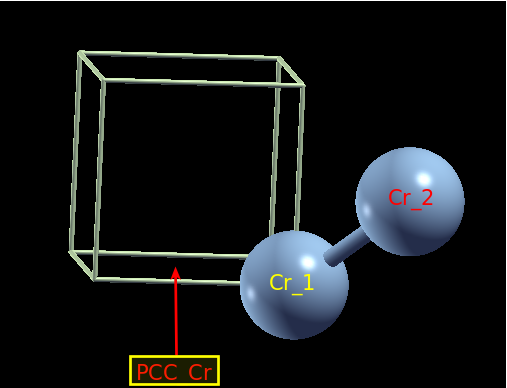
\includegraphics[height=1.20in]{Figures/WIEN2k_AFM_Cr-2.png}}
%\caption{\tiny \textrm{The structure of TiC.}}%(与文献\cite{EPJB33-47_2003}图1对比)
\end{figure}
}

\frame
{
	\frametitle{\textrm{WIEN2k}计算示范:~\ch{\textrm{Cr}}的反铁磁计算}
\vspace*{-12pt}
\begin{figure}[h!]
\centering
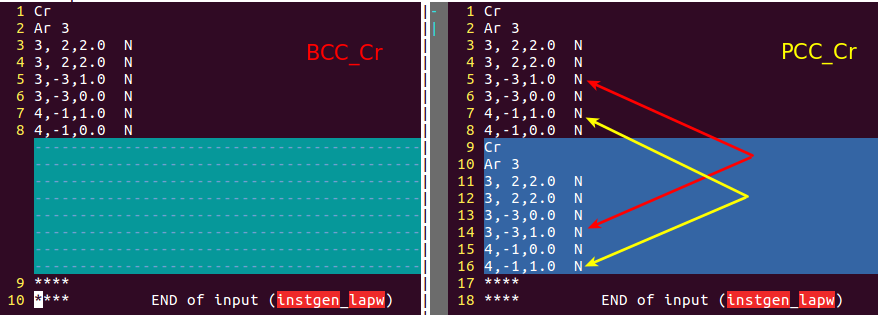
\includegraphics[width=3.7in]{Figures/WIEN2k_AFM_Cr-3.png}
\caption{\tiny \textrm{case.inst}}%(与文献\cite{EPJB33-47_2003}图1对比)
\label{Fig:WIEN2k_AFM-Cr-3}
\end{figure}
\begin{figure}[h!]
\centering
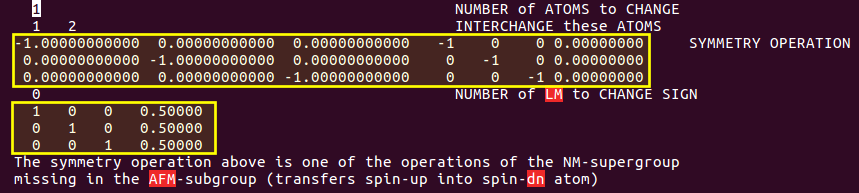
\includegraphics[width=3.50in]{Figures/WIEN2k_AFM_Cr-4.png}
\caption{\tiny \textrm{case.inclmcopy}}%(与文献\cite{EPJB33-47_2003}图1对比)
\label{Fig:WIEN2k_AFM-Cr-4}
\end{figure}
}

\frame
{
	\frametitle{\textrm{WIEN2k}计算示范:~\ch{\textrm{Cr}}的反铁磁计算}
\vspace*{-8pt}
\begin{figure}[h!]
\centering
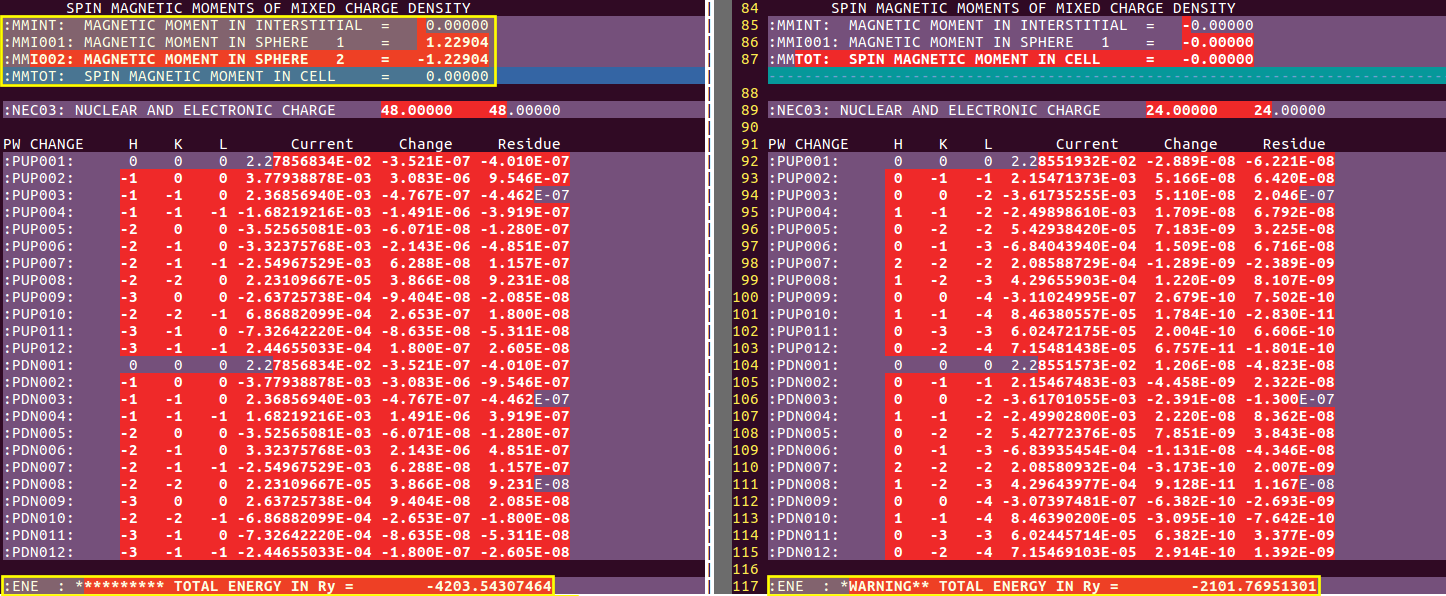
\includegraphics[width=4.1in]{Figures/WIEN2k_AFM_Cr-6.png}
%\caption{\tiny \textrm{The structure of TiC.}}%(与文献\cite{EPJB33-47_2003}图1对比)
\label{Fig:WIEN2k_AFM-Cr-6}
\end{figure}
{\fontsize{8.2pt}{6.2pt}\selectfont{
$E_{\mathrm{AFM}}$:
\begin{displaymath}
	\begin{aligned}
		&-4203.54307464-2\times(-2101.76951301)\\
		=&-0.0405~\mathrm{Ry}\\
		=&-0.11~\mathrm{eV}
	\end{aligned}
\end{displaymath} }}
}

\frame
{
	\frametitle{\textrm{WIEN2k}计算示范:~\ch{\textrm{EuB6}}的\textrm{LDA+$U$}计算}
\vspace*{-2pt}
\begin{figure}[h!]
\centering
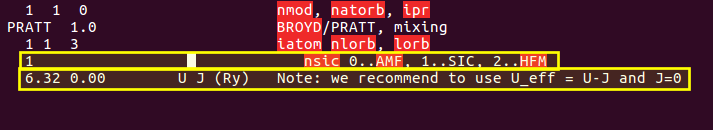
\includegraphics[width=3.7in]{Figures/WIEN2k_EuB6-inorb.png}
\caption{\tiny \textrm{case.inorb}}%(与文献\cite{EPJB33-47_2003}图1对比)
\label{Fig:WIEN2k_EuB6-inbor}
\end{figure}
\begin{figure}[h!]
\centering
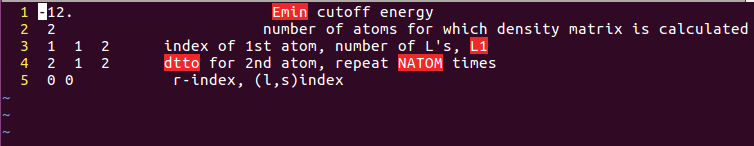
\includegraphics[width=3.70in]{Figures/WIEN2k-indm.png}
\caption{\tiny \textrm{case.indm}}%(与文献\cite{EPJB33-47_2003}图1对比)
\label{Fig:WIEN2k_indm}
\end{figure}
}

\frame
{
	\frametitle{\textrm{WIEN2k}计算示范:~\ch{\textrm{EuB6}}的\textrm{LDA+$U$}计算}
\vspace*{-10pt}
\begin{figure}[h!]
\centering
\subfigure[]{
\label{Fig:WIEN2k_EuB6-up}
	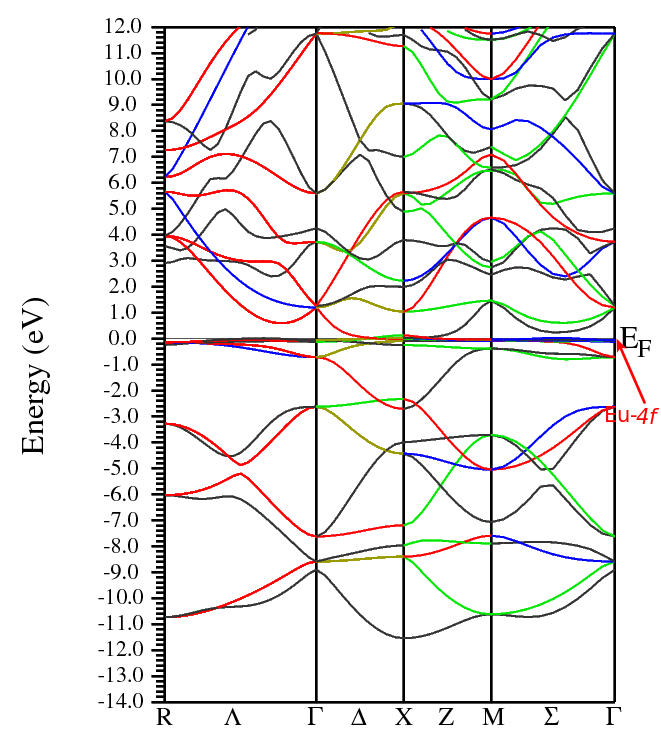
\includegraphics[height=2.15in]{Figures/WIEN2k_EuB6-band-up.png}}
	\subfigure[]{
\label{Fig:WIEN2k_EuB6-orb-up}
	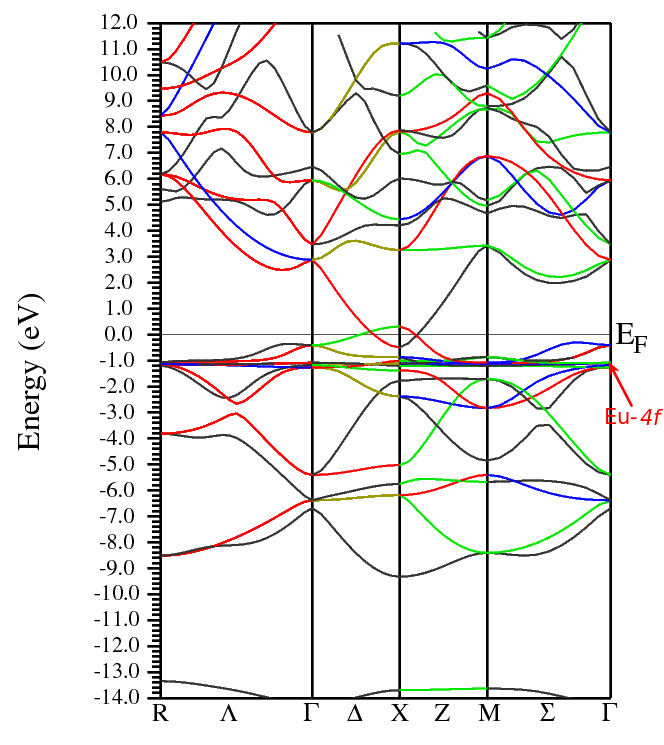
\includegraphics[height=2.15in]{Figures/WIEN2k_EuB6-band_orb-up.png}}
	\caption{\tiny \textrm{The spin-up band-structure of \ch{EuB6}.}}%(与文献\cite{EPJB33-47_2003}图1对比)
\end{figure}
}

\frame
{
	\frametitle{\textrm{WIEN2k}计算示范:~\ch{\textrm{EuB6}}的\textrm{LDA+$U$}计算}
\vspace*{-10pt}
\begin{figure}[h!]
\centering
\subfigure[]{
\label{Fig:WIEN2k_EuB6-dn}
	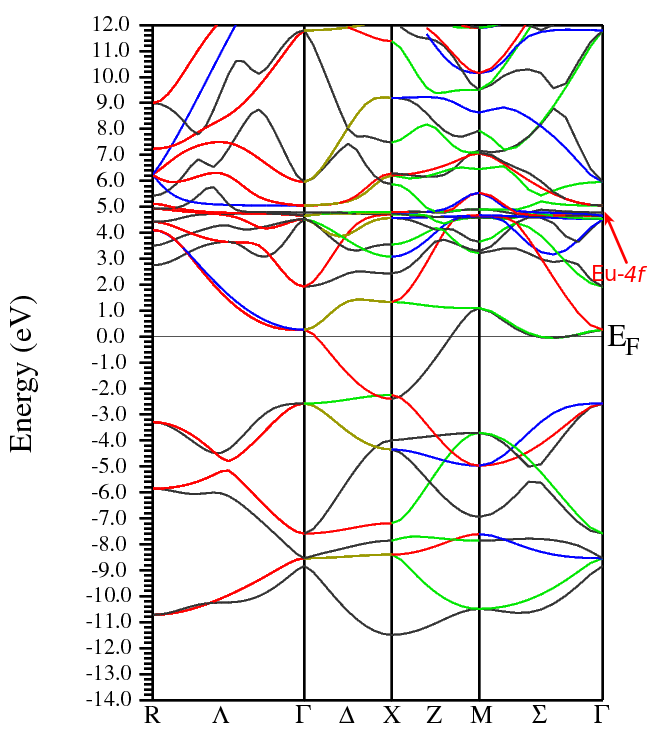
\includegraphics[height=2.15in]{Figures/WIEN2k_EuB6-band-dn.png}}
	\subfigure[]{
\label{Fig:WIEN2k_EuB6-orb-dn}
	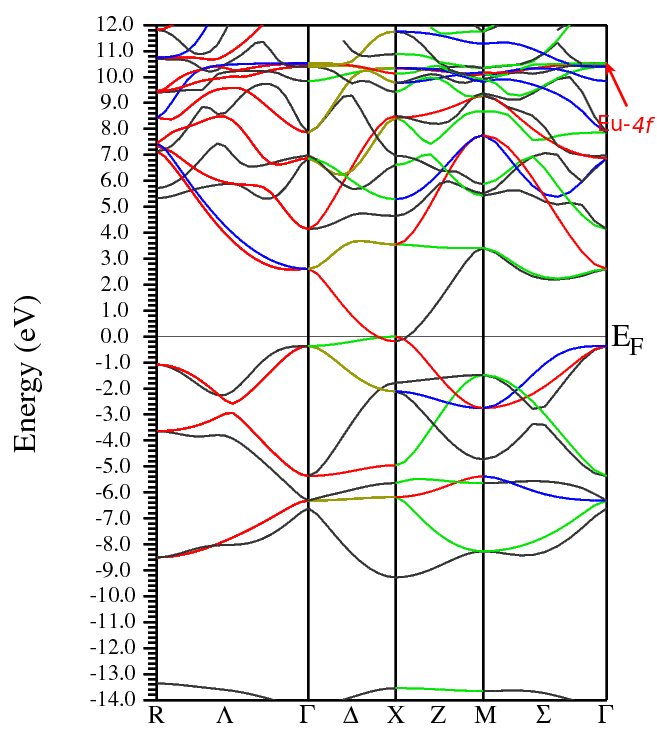
\includegraphics[height=2.15in]{Figures/WIEN2k_EuB6-band_orb-dn.png}}
	\caption{\tiny \textrm{The spin-dn band-structure of \ch{EuB6}.}}%(与文献\cite{EPJB33-47_2003}图1对比)
\end{figure}
}

\frame
{
	\frametitle{\textrm{WIEN2k}计算示范:~光学性质计算}
\vspace*{-10pt}
\begin{figure}[h!]
\centering
\subfigure[\tiny{\textrm{case.inop}}]{
\label{Fig:WIEN2k_inop}
	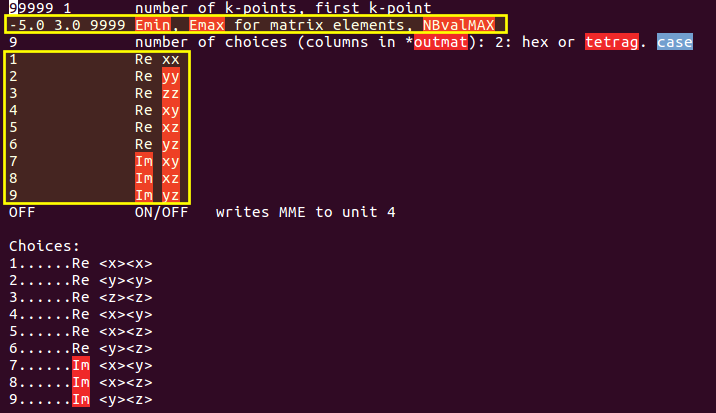
\includegraphics[height=1.25in]{Figures/WIEN2k_EuB6-inop.png}}\\
\subfigure[\tiny{\textrm{case.injoint}}]{
\label{Fig:WIEN2k_injoint}
	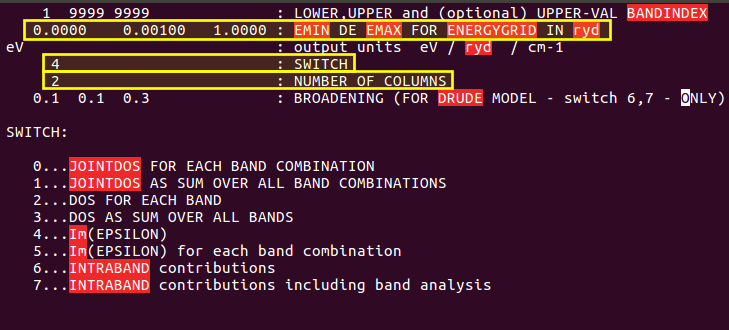
\includegraphics[height=0.95in]{Figures/WIEN2k_EuB6-injoint.png}}
	\subfigure[\tiny{\textrm{case.inkram}}]{
\label{Fig:WIEN2k_inkram}
	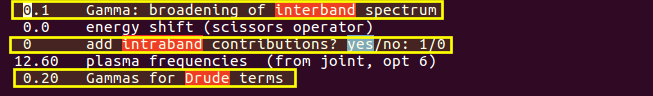
\includegraphics[height=0.26in]{Figures/WIEN2k_EuB6-inkram.png}}
%\caption{\tiny \textrm{The structure of TiC.}}%(与文献\cite{EPJB33-47_2003}图1对比)
\end{figure}
}

\frame
{
	\frametitle{\textrm{WIEN2k}计算示范:~光学性质计算}
\vspace*{-5pt}
\begin{figure}[h!]
\centering
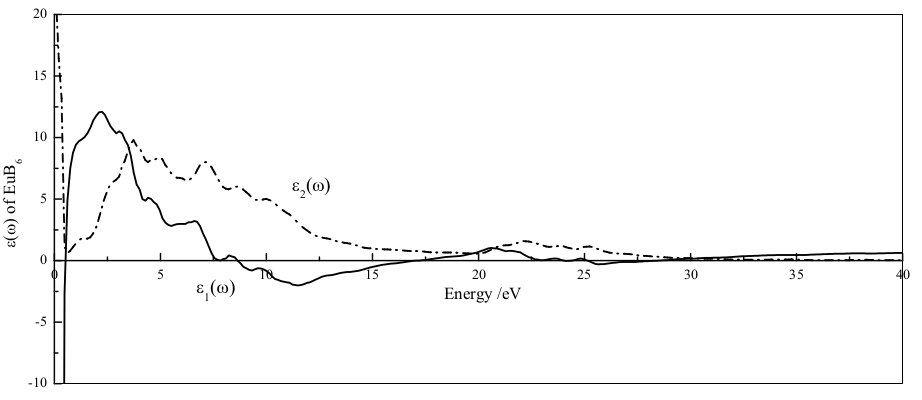
\includegraphics[width=4.15in]{Figures/WIEN2k_EuB6-epsil.png}
\caption{\tiny \textrm{The dielectric of \ch{EuB6}.}}%(与文献\cite{EPJB33-47_2003}图1对比)
\label{Fig:WIEN2k_EuB6-dielectric}
\end{figure}
}

\frame
{
	\frametitle{\textrm{WIEN2k}计算示范:~光学性质计算}
\vspace*{-5pt}
\begin{figure}[h!]
\centering
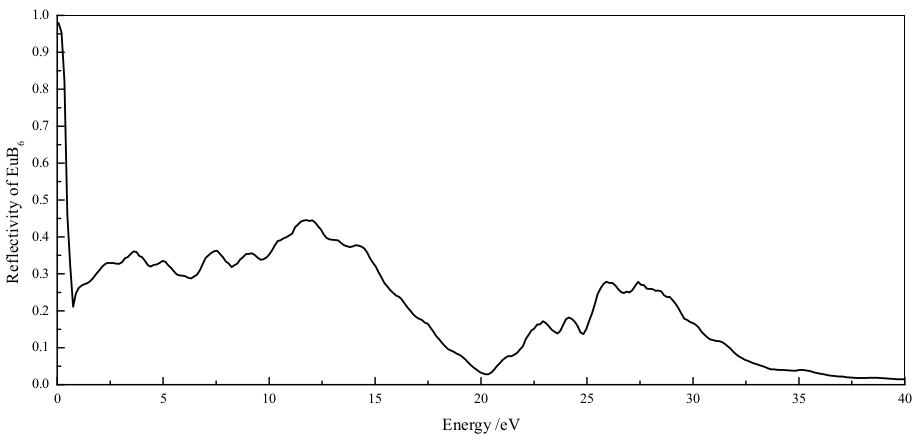
\includegraphics[width=4.15in]{Figures/WIEN2k_EuB6-Reflect.png}
\caption{\tiny \textrm{The Reflectivity of \ch{EuB6}.}}%(与文献\cite{EPJB33-47_2003}图1对比)
\label{Fig:WIEN2k_EuB6-Reflectivity}
\end{figure}
}

\frame
{
	\frametitle{\textrm{WIEN2k}计算示范:~光学性质计算}
\vspace*{-5pt}
\begin{figure}[h!]
\centering
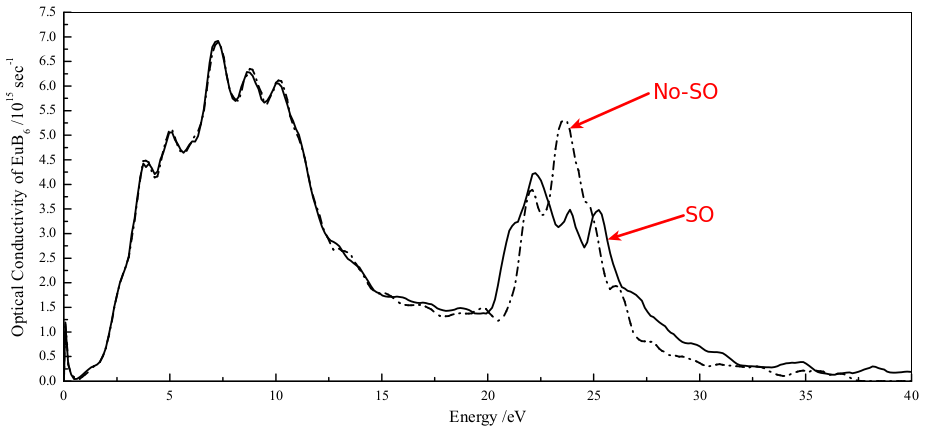
\includegraphics[width=4.15in]{Figures/WIEN2k_EuB6-Conduct.png}
\caption{\tiny \textrm{The R-conductivity of \ch{EuB6}.}}%(与文献\cite{EPJB33-47_2003}图1对比)
\label{Fig:WIEN2k_EuB6-conductivity}
\end{figure}
}

\frame
{
	\frametitle{\textrm{WIEN2k}计算示范:~光学性质计算}
\vspace*{-5pt}
\begin{figure}[h!]
\centering
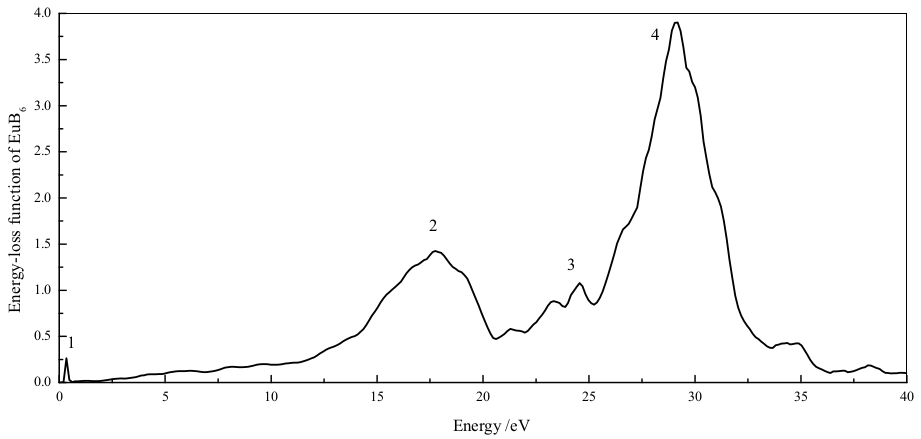
\includegraphics[width=4.15in]{Figures/WIEN2k_EuB6-eloss.png}
\caption{\tiny \textrm{The E-loss function of \ch{EuB6}.}}%(与文献\cite{EPJB33-47_2003}图1对比)
\label{Fig:WIEN2k_EuB6-eloss}
\end{figure}
%\vskip 5pt
%\tiny{\textcolor{blue}{以上全部算例未作特别说明,均引自文献\cite{Jun_Jiang}}}
}

\frame
{
	\frametitle{\textrm{WIEN2k}计算示范:~\ch{\textrm{EuB6}}的\textrm{SOC}计算}
\vspace*{-5pt}
\begin{figure}[h!]
\centering
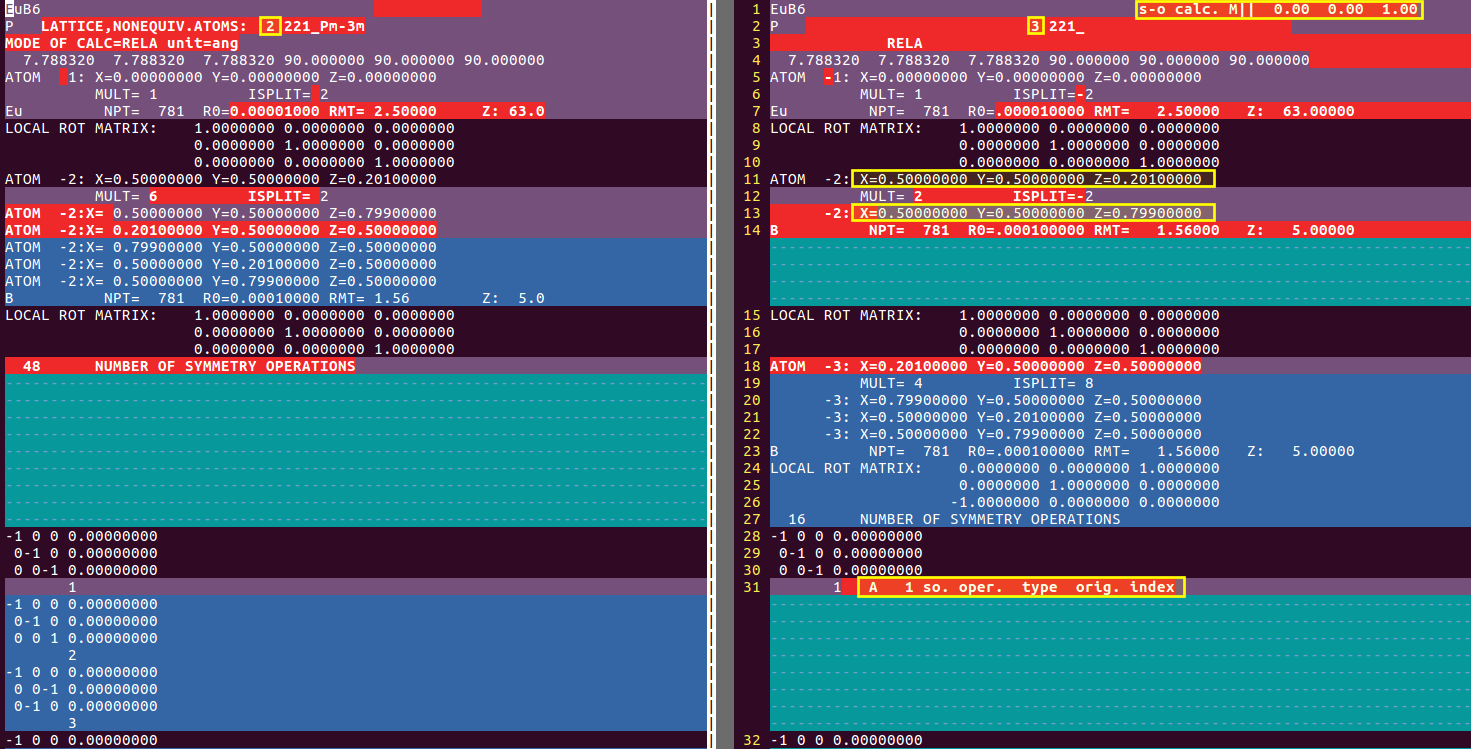
\includegraphics[width=4.15in]{Figures/WIEN2k_EuB6-struct-so.png}
\caption{\tiny \textrm{The structure of \ch{EuB6}.}}%(与文献\cite{EPJB33-47_2003}图1对比)
\label{Fig:WIEN2k_SOC-struct}
\end{figure}
}

\frame
{
	\frametitle{\textrm{WIEN2k}计算示范:~\ch{\textrm{EuB6}}的\textrm{SOC}计算}
\vspace*{-10pt}
\begin{minipage}[t]{0.39\textwidth}
\begin{figure}[h!]
\centering
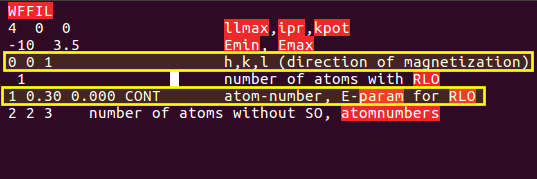
\includegraphics[width=1.65in]{Figures/WIEN2k_EuB6-inso.png}
\caption{\tiny \textrm{case.inso}}%(与文献\cite{EPJB33-47_2003}图1对比)
\label{Fig:WIEN2k_EuB6-inso}
\end{figure}
\end{minipage}
\hfill
\begin{minipage}[t]{0.59\textwidth}
\begin{figure}[h!]
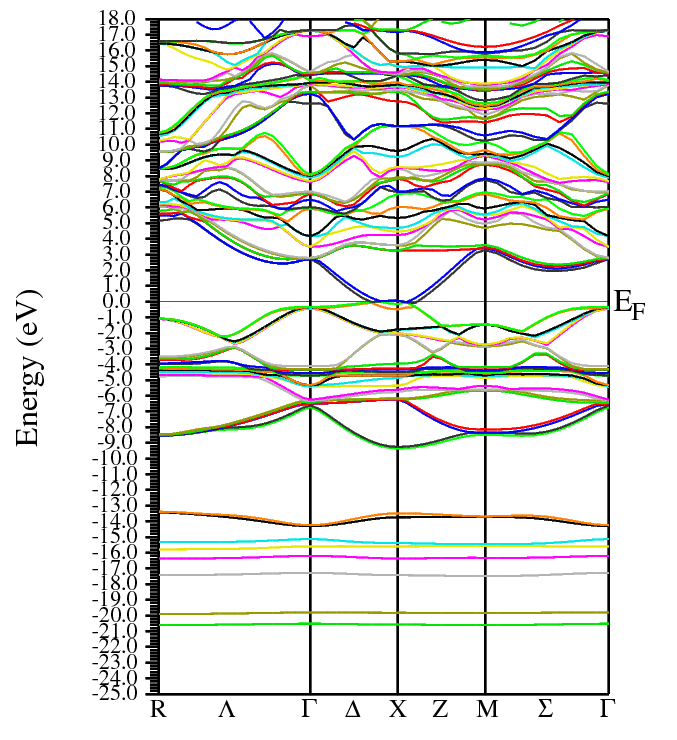
\includegraphics[height=2.70in]{Figures/WIEN2k_EuB6-band_orb_so.png}
%\caption{\tiny Breakup of a submesh cell into six tetrahedra.}%(与文献\cite{EPJB33-47_2003}图1对比)
\label{Fig:WIEN2k_EuB6-band-SO}
\end{figure}
\end{minipage}
}
